\documentclass{article}
\usepackage{amsmath}
\usepackage{amsthm}
\usepackage{graphicx}
\usepackage{tikz}
\usepackage{pgfplots}
\pgfplotsset{compat=1.18}
\usepackage{booktabs}
\usepackage{enumitem}
\usepackage[margin=1in]{geometry}
\usepackage{titlesec}

\titleformat{\section}[block]{\normalfont\large\bfseries\centering}{\thesection}{1em}{}
\titleformat{\subsection}[block]{\normalfont\bfseries\centering}{\thesubsection}{1em}{}

\theoremstyle{definition}
\newtheorem{definition}{Definition}
\newtheorem{example}{Example}

\title{Study Notes: Chapter 1 - Describing Data with Graphs}
\author{Professor and Academic Researcher}
\date{}

\begin{document}
	
	\maketitle
	
	\section{Introduction to Chapter 1}
	This chapter focuses on descriptive statistics, specifically using graphs to summarize and visualize data. We explore variables, data types, and graphical representations for categorical and quantitative data. Understanding these tools helps reveal patterns, trends, and insights in datasets. Many examples are drawn from real-world applications, such as surveys, medical data, and population statistics.
	
	\section{1.1 Variables and Data}
	Data description begins with understanding variables and how data are generated. Variables are characteristics that vary across time or individuals, and data are the measurements obtained from these variables.
	
	\subsection{Key Definitions}
	
	\begin{definition}[Variable]
		A variable is a characteristic that changes or varies over time and/or for different individuals or objects under consideration. For instance, body temperature varies over time for an individual and differs between people.
	\end{definition}
	
	\begin{definition}[Experimental Unit]
		An experimental unit is the individual or object on which a variable is measured. Examples include a student for GPA measurement or a patient for blood pressure.
	\end{definition}
	
	\begin{definition}[Measurement or Data Value]
		A measurement or data value is the result when a variable is measured on an experimental unit. For example, measuring height yields a specific number like 1.75 meters.
	\end{definition}
	
	\begin{definition}[Population]
		A population is the set of all measurements of interest to the investigator. It could be all body temperatures of healthy humans worldwide.
	\end{definition}
	
	\begin{definition}[Sample]
		A sample is a subset of measurements selected from the population. Due to practical constraints, we often work with samples to infer about populations.
	\end{definition}
	
	\begin{definition}[Univariate Data]
		Univariate data results from measuring a single variable on an experimental unit, e.g., heights of 100 people.
	\end{definition}
	
	\begin{definition}[Bivariate and Multivariate Data]
		Bivariate data involves two variables per unit, e.g., height and weight. Multivariate data involves more than two, as in student records with GPA, gender, year, major, and units.
	\end{definition}
	\newpage
	\subsection{Types of Variables}
	
	Variables are classified as qualitative (categorical) or quantitative (numerical). Quantitative variables are further divided into discrete or continuous.
	
	\begin{definition}[Qualitative Variable]
		Qualitative variables measure a quality or characteristic, producing categorical data. Examples: gender (male/female), political affiliation (Republican/Democrat/Independent).
	\end{definition}
	
	\begin{definition}[Quantitative Variable]
		Quantitative variables measure a numerical quantity. Examples: height, weight, number of siblings.
	\end{definition}
	
	\begin{definition}[Discrete Variable]
		Discrete variables assume a finite or countable number of values, often involving counts. Examples: number of children (0, 1, 2, ...), number of defective items.
	\end{definition}
	
	\begin{definition}[Continuous Variable]
		Continuous variables assume infinitely many values on a line interval. Examples: time, distance, volume—any value between two points is possible.
	\end{definition}
	
	Detailed Explanation: Qualitative data categorize observations without numerical values, useful for grouping. Quantitative data allow arithmetic operations. Discrete data have gaps (e.g., no 1.5 children), while continuous data do not (e.g., weight can be 70.5 kg).
	
	\subsection{Examples}
	
	\begin{example}
		Measurements on five undergraduates: GPA, gender, year, major, units (Figure 1.1 in book). This is multivariate data. GPA and units are quantitative (GPA continuous, units discrete); gender, year, major qualitative.
		
		Here is Figure 1.1 recreated as a table:
		
		\begin{table}[ht]
			\centering
			\begin{tabular}{cccccc}
				\toprule
				Student & GPA & Gender & Year & Major & \# of Units \\
				\midrule
				1 & 3.1 & M & Fr & Psychology & 13 \\
				2 & 2.3 & F & So & Mathematics & 15 \\
				3 & 3.9 & M & So & English & 17 \\
				4 & 2.7 & M & Fr & Business & 15 \\
				5 & 2.4 & F & Jr & English & 16 \\
				\bottomrule
			\end{tabular}
			\caption{Measurements on five undergraduate students}
		\end{table}
	\end{example}
	
	\begin{example}
		Classify: Microwave use (qualitative), survey refusals (discrete quantitative), mouse door choice (qualitative), horse winning time (continuous quantitative), children reading at grade level (discrete quantitative).
	\end{example}
	\newpage
	\section{1.2 Graphs for Categorical Data}
	
	Categorical data are summarized using frequencies, relative frequencies, or percentages in tables, then visualized with pie or bar charts.
	
	Detailed Explanation: Frequencies count occurrences per category. Relative frequency = frequency / n, percentage = relative frequency × 100. Categories must be mutually exclusive and exhaustive.
	
	\subsection{Graphs}
	
	\textbf{Pie Chart}: Shows proportions as sectors of a circle. Angle = relative frequency × 360°.
	
	\textbf{Bar Chart}: Heights represent frequencies/percentages. Pareto chart orders bars descending.
	
	\begin{example}[U.S. Education Rating]
		Ratings: A (35), B (260), C (93), D (12). Pie chart sectors: A 32.4°, B 234°, C 82.8°, D 10.8° (Figure 1.3). Bar chart heights match frequencies (Figure 1.4). Pie emphasizes proportions, bar actual counts.
		
		Here is a visualization of the pie chart:
		
		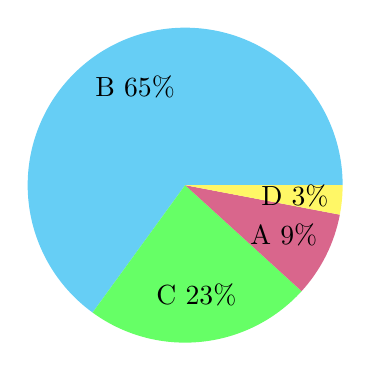
\begin{tikzpicture}
			\def\currentangle{0}
			\fill[cyan!60] (0,0) -- ++(\currentangle:2) 
			arc[start angle=\currentangle, end angle={\currentangle+234}, radius=2] -- cycle;
			\node at ({ \currentangle + 117 }:1.4) {B 65\%};
			
			\pgfmathsetmacro{\currentangle}{\currentangle + 234}
			\fill[green!60] (0,0) -- ++(\currentangle:2) 
			arc[start angle=\currentangle, end angle={\currentangle+83.7}, radius=2] -- cycle;
			\node at ({ \currentangle + 41.85 }:1.4) {C 23\%};
			
			\pgfmathsetmacro{\currentangle}{\currentangle + 83.7}
			\fill[purple!60] (0,0) -- ++(\currentangle:2) 
			arc[start angle=\currentangle, end angle={\currentangle+31.5}, radius=2] -- cycle;
			\node at ({ \currentangle + 15.75 }:1.4) {A 9\%};
			
			\pgfmathsetmacro{\currentangle}{\currentangle + 31.5}
			\fill[yellow!60] (0,0) -- ++(\currentangle:2) 
			arc[start angle=\currentangle, end angle={\currentangle+10.8}, radius=2] -- cycle;
			\node at ({ \currentangle + 5.4 }:1.4) {D 3\%};
		\end{tikzpicture}
		
		Here is a visualization of the bar chart:
		
		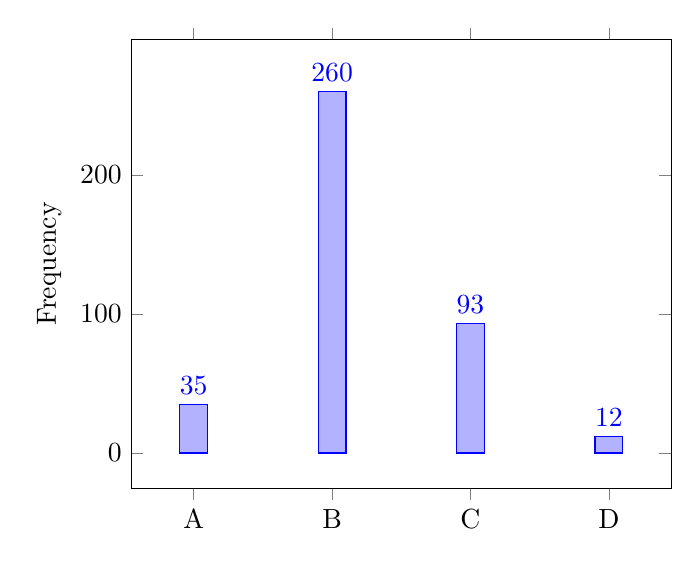
\begin{tikzpicture}
			\begin{axis}[
				ybar,
				enlargelimits=0.15,
				ylabel={Frequency},
				symbolic x coords={A,B,C,D},
				xtick=data,
				nodes near coords,
				nodes near coords align={vertical},
				]
				\addplot coordinates {(A,35) (B,260) (C,93) (D,12)};
			\end{axis}
		\end{tikzpicture}
	\end{example}
	
	\begin{example}[M\&M Colors]
		Colors in bag: Brown (6), Green (3), Orange (3), Yellow (2), Red (2), Blue (5). Pareto chart: Brown, Blue, Green, Orange, Yellow, Red (Figure 1.5).
		
		Here is a visualization of the Pareto chart:
		
		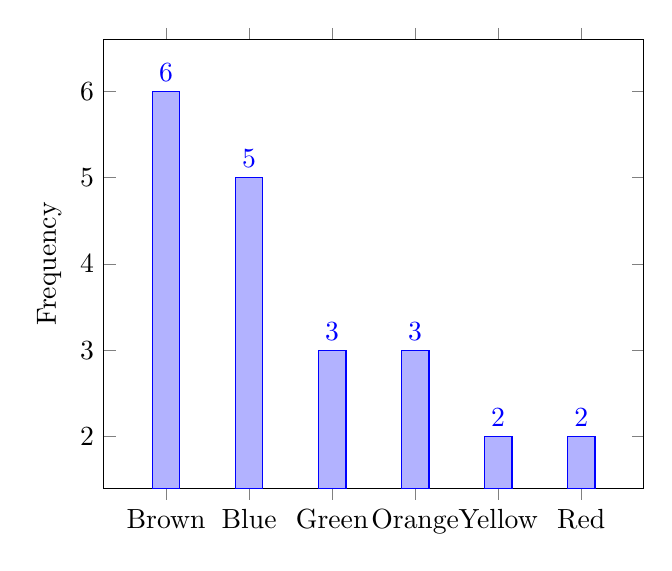
\begin{tikzpicture}
			\begin{axis}[
				ybar,
				enlargelimits=0.15,
				ylabel={Frequency},
				symbolic x coords={Brown,Blue,Green,Orange,Yellow,Red},
				xtick=data,
				nodes near coords,
				nodes near coords align={vertical},
				]
				\addplot coordinates {(Brown,6) (Blue,5) (Green,3) (Orange,3) (Yellow,2) (Red,2)};
			\end{axis}
		\end{tikzpicture}
	\end{example}
	
	\section{1.3 Graphs for Quantitative Data}
	
	Quantitative data graphs include pie/bar for categorized data, line for time series, dotplots, stem and leaf for raw data.
	
	\subsection{Pie Charts and Bar Charts for Quantitative Data}
	
	Used when quantitative data are grouped, e.g., expenses by category.
	
	\begin{example}[Defense Expenses]
		Categories: Personnel (138.6), Operations (244.4), Procurement (118.9), Research and development (69.0), Military construction (6.9), Other (2.5) (Table 1.5). Bar chart shows amounts (Figure 1.6), pie proportions (Figure 1.7). Operations largest slice/bar.
		
		Here is Table 1.5:
		
		\begin{table}[ht]
			\centering
			\begin{tabular}{lr}
				\toprule
				Category & Amount (\$ billions) \\
				\midrule
				Military personnel & 138.6 \\
				Operation and maintenance & 244.4 \\
				Procurement & 118.9 \\
				Research and development & 69.0 \\
				Military construction & 6.9 \\
				Other & 2.5 \\
				Total & 580.3 \\
				\bottomrule
			\end{tabular}
			\caption{Expenses by Category}
		\end{table}
		
		Here is a recreation of Figure 1.6 (bar chart):
		
		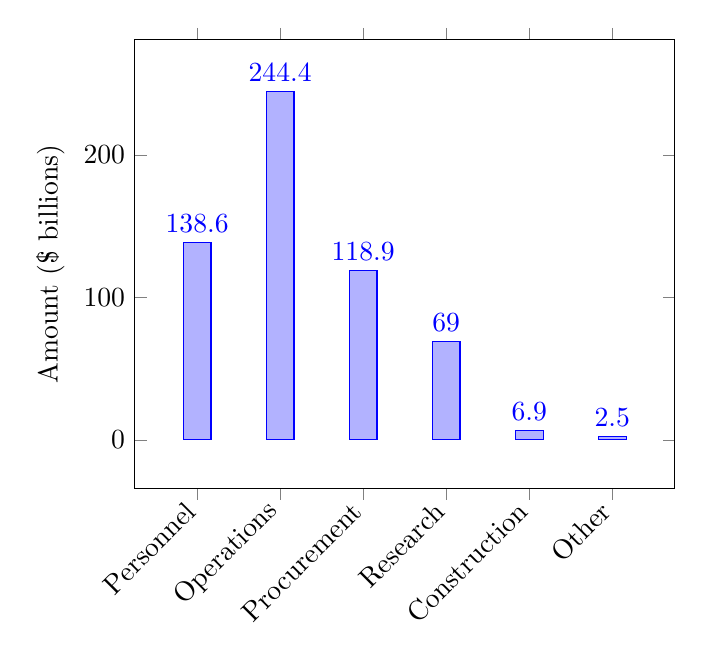
\begin{tikzpicture}
			\begin{axis}[
				ybar,
				enlargelimits=0.15,
				ylabel={Amount (\$ billions)},
				symbolic x coords={Personnel,Operations,Procurement,Research,Construction,Other},
				xtick=data,
				xticklabels={Personnel,Operations,Procurement,Research,Construction,Other},
				nodes near coords,
				nodes near coords align={vertical},
				x tick label style={rotate=45,anchor=east},
				]
				\addplot coordinates {(Personnel,138.6) (Operations,244.4) (Procurement,118.9) (Research,69.0) (Construction,6.9) (Other,2.5)};
			\end{axis}
		\end{tikzpicture}
		
		Here is a recreation of Figure 1.7 (pie chart):
		
		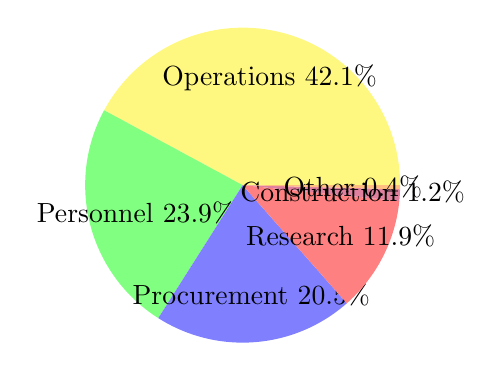
\begin{tikzpicture}
			\def\currentangle{0}
			\fill[yellow!50] (0,0) -- ++(\currentangle:2) 
			arc[start angle=\currentangle, end angle={\currentangle + 151.6}, radius=2] -- cycle;
			\node at ({ \currentangle + 75.8 }:1.4) {Operations 42.1\%};
			
			\pgfmathsetmacro{\currentangle}{\currentangle + 151.6}
			\fill[green!50] (0,0) -- ++(\currentangle:2) 
			arc[start angle=\currentangle, end angle={\currentangle + 86.0}, radius=2] -- cycle;
			\node at ({ \currentangle + 43 }:1.4) {Personnel 23.9\%};
			
			\pgfmathsetmacro{\currentangle}{\currentangle + 86.0}
			\fill[blue!50] (0,0) -- ++(\currentangle:2) 
			arc[start angle=\currentangle, end angle={\currentangle + 73.8}, radius=2] -- cycle;
			\node at ({ \currentangle + 36.9 }:1.4) {Procurement 20.5\%};
			
			\pgfmathsetmacro{\currentangle}{\currentangle + 73.8}
			\fill[red!50] (0,0) -- ++(\currentangle:2) 
			arc[start angle=\currentangle, end angle={\currentangle + 42.8}, radius=2] -- cycle;
			\node at ({ \currentangle + 21.4 }:1.4) {Research 11.9\%};
			
			\pgfmathsetmacro{\currentangle}{\currentangle + 42.8}
			\fill[purple!50] (0,0) -- ++(\currentangle:2) 
			arc[start angle=\currentangle, end angle={\currentangle + 4.3}, radius=2] -- cycle;
			\node at ({ \currentangle + 2.15 }:1.4) {Construction 1.2\%};
			
			\pgfmathsetmacro{\currentangle}{\currentangle + 4.3}
			\fill[orange!50] (0,0) -- ++(\currentangle:2) 
			arc[start angle=\currentangle, end angle={\currentangle + 1.5}, radius=2] -- cycle;
			\node at ({ \currentangle + 0.75 }:1.4) {Other 0.4\%};
		\end{tikzpicture}
	\end{example}
	
	\subsection{Line Charts}
	
	For time series, connect points over time to show trends.
	
	\begin{example}[Population 85+]
		Projections: 2020 (6.7M), 2030 (9.1M), 2040 (14.6M), 2050 (19.0M), 2060 (19.7M) (Table 1.6). Line chart shows upward trend (Figure 1.8). Scale affects perceived steepness—beware manipulation.
		
		Here is Table 1.6:
		
		\begin{table}[ht]
			\centering
			\begin{tabular}{cccccc}
				\toprule
				Year & 2020 & 2030 & 2040 & 2050 & 2060 \\
				\midrule
				85 and over (millions) & 6.7 & 9.1 & 14.6 & 19.0 & 19.7 \\
				\bottomrule
			\end{tabular}
			\caption{Population Growth Projections}
		\end{table}
		
		Here is a recreation of Figure 1.8 (line chart):
		
		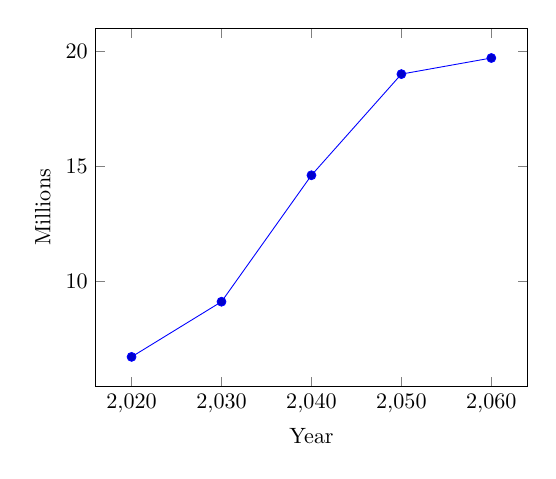
\begin{tikzpicture}[scale=0.8]
			\begin{axis}[
				xlabel={Year},
				ylabel={Millions},
				xtick={2020,2030,2040,2050,2060},
				]
				\addplot coordinates {(2020,6.7) (2030,9.1) (2040,14.6) (2050,19.0) (2060,19.7)};
			\end{axis}
		\end{tikzpicture}
	\end{example}
	
	\subsection{Dotplots}
	
	Plot measurements as dots on horizontal axis.
	
	Detailed Explanation: Simple for small sets, shows clustering/outliers. For large sets, may overlap—use stem/leaf or histogram.
	
	\begin{example}
		Small: 2,6,9,3,7,6 (Figure 1.9a). Large: Many points (Figure 1.9b)—hard to interpret.
		
		Here is a recreation of Figure 1.9a:
		
		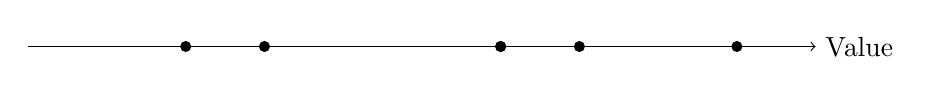
\begin{tikzpicture}
			\draw[->] (0,0) -- (10,0) node[right] {Value};
			\foreach \x in {2,3,6,6,7,9} \fill (\x,0) circle (2pt);
		\end{tikzpicture}
	\end{example}
	
	\subsection{Stem and Leaf Plots}
	
	Uses digits: stem (leading), leaf (trailing).
	
	\begin{example}[Shoe Prices]
		Prices: 90, 70, 70, 70, 75, 70, 65, 68, 60, 74, 70, 95, 75, 70, 68, 65, 40, 65, 70 (Table 1.7). Stems 4-9, leaves sorted (Figure 1.10).
		
		Here is Figure 1.10 (stem and leaf plot):
		
		{\small
			\begin{verbatim}
				4 | 0
				5 | 
				6 | 0 5 5 5 8 8
				7 | 0 0 0 0 0 4 5 5 5
				8 | 
				9 | 0 5
				Leaf unit = 1
			\end{verbatim}
		}
		
	\end{example}
	
	\begin{example}[Birth Weights]
		Weights: 7.2, 7.8, 6.8, 6.2, 8.2, 8.0, 8.2, 5.6, 8.6, 7.1, 8.2, 7.7, 7.5, 7.2, 7.7, 5.8, 6.8, 6.8, 8.5, 7.5, 6.1, 7.9, 9.4, 9.0, 7.8, 8.5, 9.0, 7.7, 6.7, 7.7 (Table 1.8). Divided stems for detail, mound-shaped (Figure 1.11).
		
		Here is Figure 1.11 (stem and leaf plot):
		
		{\small
			\begin{verbatim}
				5 | 6 8
				6 | 1 2 2
				6 | 8 8 8
				7 | 1 2 2
				7 | 5 5 7 7 7 8 9
				8 | 0 2 2 2 5 5
				8 | 5 6
				9 | 0 0 4
				Leaf unit = 0.1
			\end{verbatim}
		}
		
	\end{example}
	
	\subsection{Interpreting Graphs with a Critical Eye}
	
	Examine scale, location (center), shape (symmetric/skewed, uni/bimodal), outliers.
	
	Detailed Explanation: Symmetric: mirror halves. Skewed right: long right tail, few large values. Skewed left: long left tail, few small values. Unimodal: one peak. Bimodal: two peaks (mixed populations). Outliers: extreme values—check validity.
	
	\begin{example}
		Dotplots: Symmetric mound (a), uniform (b), skewed right (c), skewed left (d) (Figure 1.12).
		
		Here is a recreation of Figure 1.12:
		
		(a) Symmetric mound:
		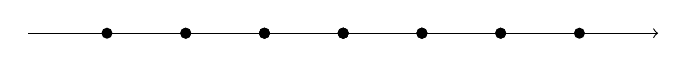
\begin{tikzpicture}
			\draw[->] (0,0) -- (8,0);
			\foreach \x in {1,2,2,3,3,3,4,4,4,4,5,5,5,6,6,7} \fill (\x,0) circle (2pt);
		\end{tikzpicture}
		
		(b) Uniform:
		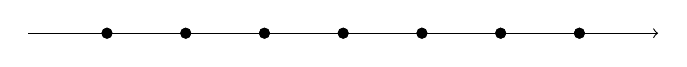
\begin{tikzpicture}
			\draw[->] (0,0) -- (8,0);
			\foreach \x in {1,1,2,2,3,3,4,4,5,5,6,6,7,7} \fill (\x,0) circle (2pt);
		\end{tikzpicture}
		
		(c) Skewed right:
		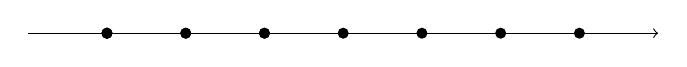
\begin{tikzpicture}
			\draw[->] (0,0) -- (8,0);
			\foreach \x in {1,1,1,2,2,3,3,4,5,6,7} \fill (\x,0) circle (2pt);
		\end{tikzpicture}
		
		(d) Skewed left:
		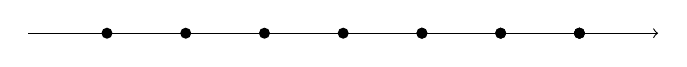
\begin{tikzpicture}
			\draw[->] (0,0) -- (8,0);
			\foreach \x in {1,2,3,4,5,5,6,6,7,7,7} \fill (\x,0) circle (2pt);
		\end{tikzpicture}
	\end{example}
	
	\begin{example}[GPAs with Error]
		GPAs: 2.8, 3.0, 3.0, 3.3, 2.4, 3.4, 3.0, 0.21. Dotplot shows outlier at 0.21—data entry error (Figure 1.13).
		
		Here is a recreation of Figure 1.13(a):
		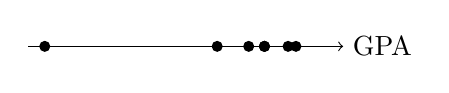
\begin{tikzpicture}
			\draw[->] (0,0) -- (4,0) node[right] {GPA};
			\foreach \x in {0.21,2.4,2.8,3.0,3.0,3.0,3.3,3.4} \fill (\x,0) circle (2pt);
		\end{tikzpicture}
		
		(b) Corrected (0.21 to 2.1):
		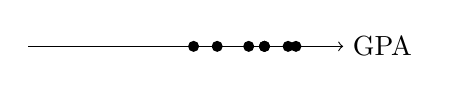
\begin{tikzpicture}
			\draw[->] (0,0) -- (4,0) node[right] {GPA};
			\foreach \x in {2.1,2.4,2.8,3.0,3.0,3.0,3.3,3.4} \fill (\x,0) circle (2pt);
		\end{tikzpicture}
	\end{example}
	
	\section{1.4 Relative Frequency Histograms}
	
	Bar graph for quantitative data: classes on x-axis, relative frequencies on y-axis.
	
	Detailed Explanation: Classes: equal-width subintervals. Boundaries avoid data points. Width: upper - lower boundary. Frequency: counts per class. Relative frequency histogram shows proportions.
	
	Guidelines: 5-20 classes, equal width, exhaustive.
	
	\begin{example}[Birth Weights]
		Classes: 5.0-5.9,6.0-6.9,... Mound-shaped distribution (Figure 1.14c).
		
		Here is a recreation of Figure 1.14c (histogram):
		
		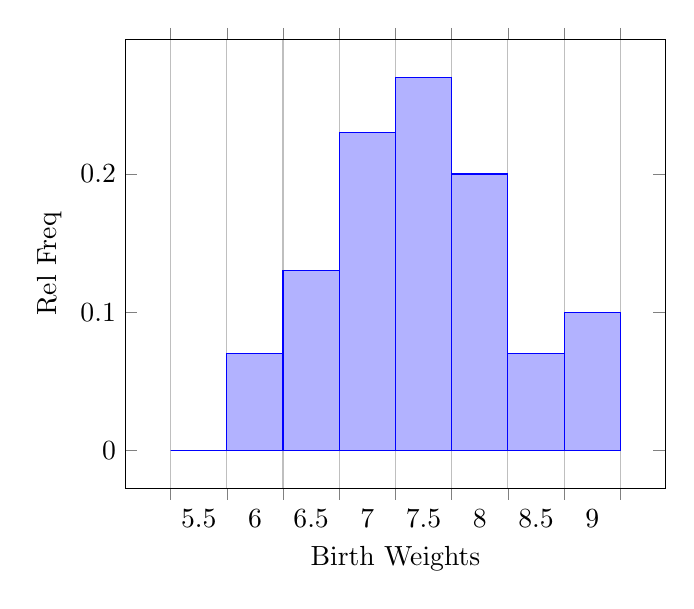
\begin{tikzpicture}
			\begin{axis}[
				ybar interval,
				xlabel={Birth Weights},
				ylabel={Rel Freq},
				]
				\addplot coordinates {(5.5,0) (6.0,0.07) (6.5,0.13) (7.0,0.23) (7.5,0.27) (8.0,0.2) (8.5,0.07) (9.0,0.1) (9.5,0)};
			\end{axis}
		\end{tikzpicture}
		(Note: Approximate frequencies based on data distribution.)
	\end{example}
\end{document}